\chapter{Approach}
% Describe the performed solution with all possible details. Define necessary parameters, inputs, outputs and context of use, possible problems and when they can be applied. 

% Remember to define necessary concepts before using them, building the text from easiest definitions (not depending on previous definitions) to complex definitions (depending on previous definitions).

% E.g: 
% \begin{itemize}
%	\item Lost Communication: a lost communication occurs when the conditions of the environment are not sufficient or the distance between sender and receiver is to hight to transmit information.
%	\item Wait until rescue: when the robot loses its communication, the pre-designed state machine will stop the motors to keep the actual position. Energy safe mode will be enabled, at the same time that a channel transceiver daemon will send SOS messages every T and wait for reply during T sec. 
%\end{itemize}
In our system there are multiple robots that must handle various tasks. For example, visiting given rooms. To tackle this problem, a communication efficient task scheduling system is designed. 
This system allocate task according to system resources, including environment factors and robot available battery. Once this information is attained, the task scheduling system assign robot a set of task.
\begin{itemize}
	\item \textsl{Robot.} The robot is responsible for moving in 2-dimensional physical space as well as listen to sensors on its way. It has a rechargeable battery. Robot battery level drops as its moves and rotates.
	\item \textsl{Tasks.} Each task requires one or more robots to traverse a path in the workspace and carry out certain actions.
	\item \textsl{Environment.} We consider robots moving in an office that contains a corridor along the central x-axis and 16 rooms located around the corridor. The environment model is shown in Figure \ref{fig:gazebo_model}. The environment factors, such as room locations and occupancy possibilities help task allocation.
\end{itemize}

\begin{figure}[htbp]
	\centering
	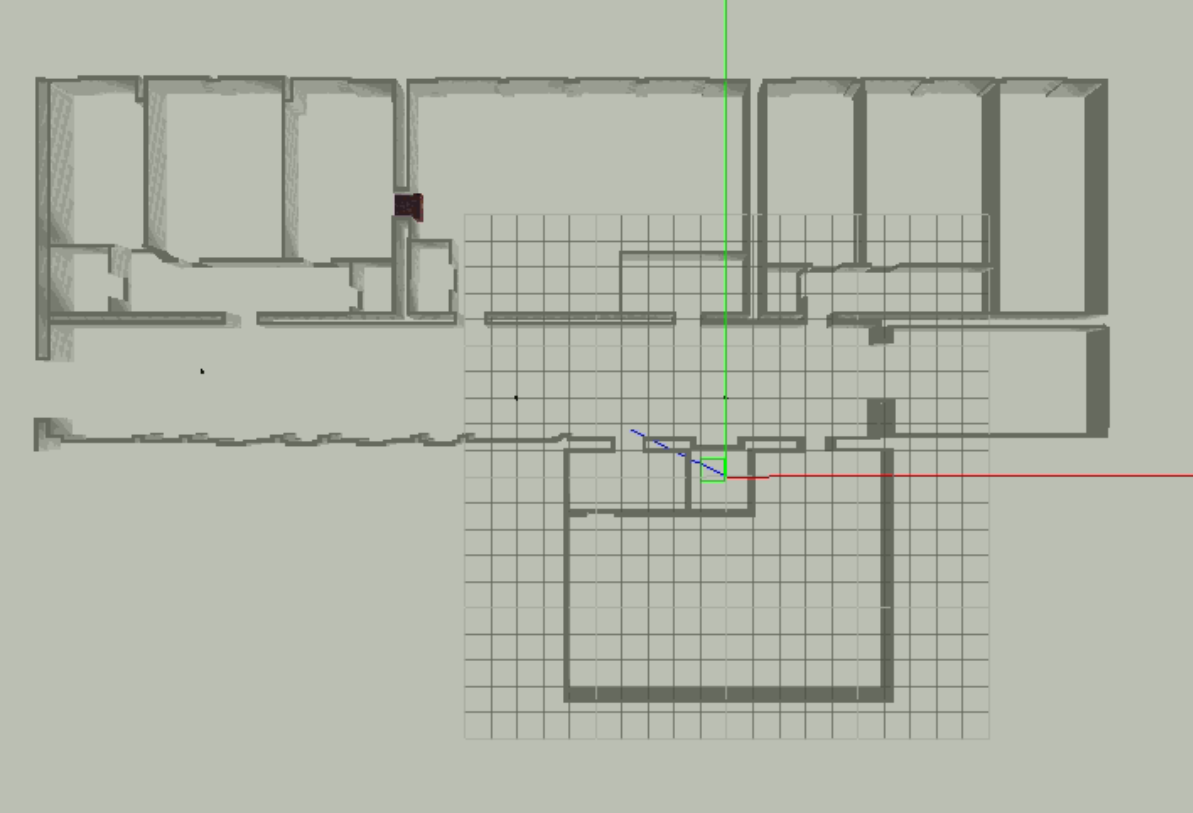
\includegraphics[width = 0.7\textwidth]{content/images/ch3/gazebo_model.png}
	\caption{Gazebo Model}
	\label{fig:gazebo_model}
\end{figure}

\section{Architecture Design}

As shown in Figure \ref{fig:system_architecture}, the architecture of the system consist of several parts: centralized pool, robot controller, navigation stack, charging station and system environment. 
\begin{itemize}
	\item \textsl{Centralized Pool.} A centralized pool consist of several modules: multi-robot task allocation module, system environment state, database, execution and monitoring. The database contains the room information such as occupancy possible and the tasks. The multi-robot task allocation module assign task to robots according to both robot status and system environment.
	\item \textsl{Robot Controller.} A robot controller contains several modules: execute module and robot action. The execute module receive commands from centralized pool and decide when and which task the robot should perform. During performing a task, a robot can send environment information to centralized pool.
	\item \textsl{Navigation stack.} The move\_base node provides a ROS interface for configuring, running, and interacting with the navigation stack on a robot. It makes robot move to desired positions using the navigation stack. Its advantages include optionally performing recovery behaviors when the robot perceives itself as stuck. 
\end{itemize} 

\begin{figure}[htbp]
	\centering
	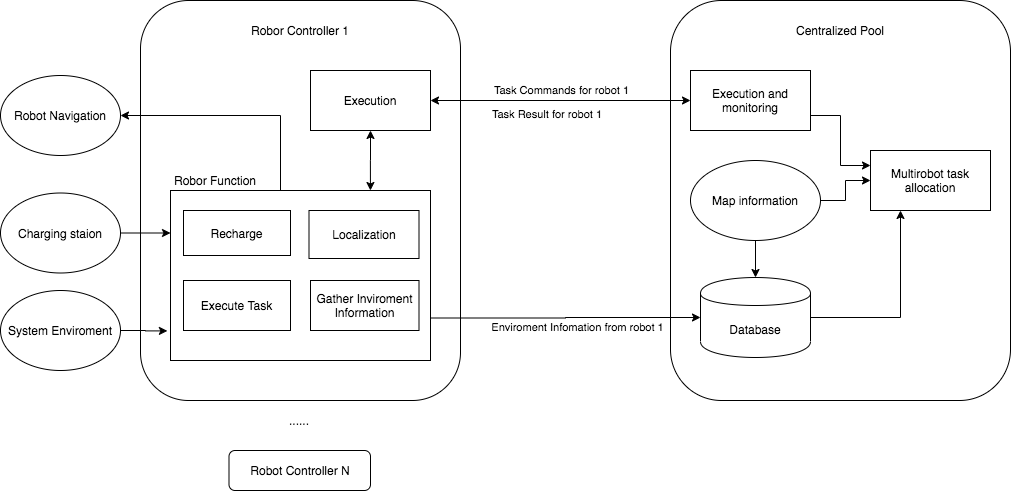
\includegraphics[width = 0.8\textwidth]{content/images/ch3/architecture.drawio.png}
	\caption{Multi-robot task allocation and execution system architecture}
	\label{fig:system_architecture}
\end{figure}

\begin{figure}[htbp]
	\centering
	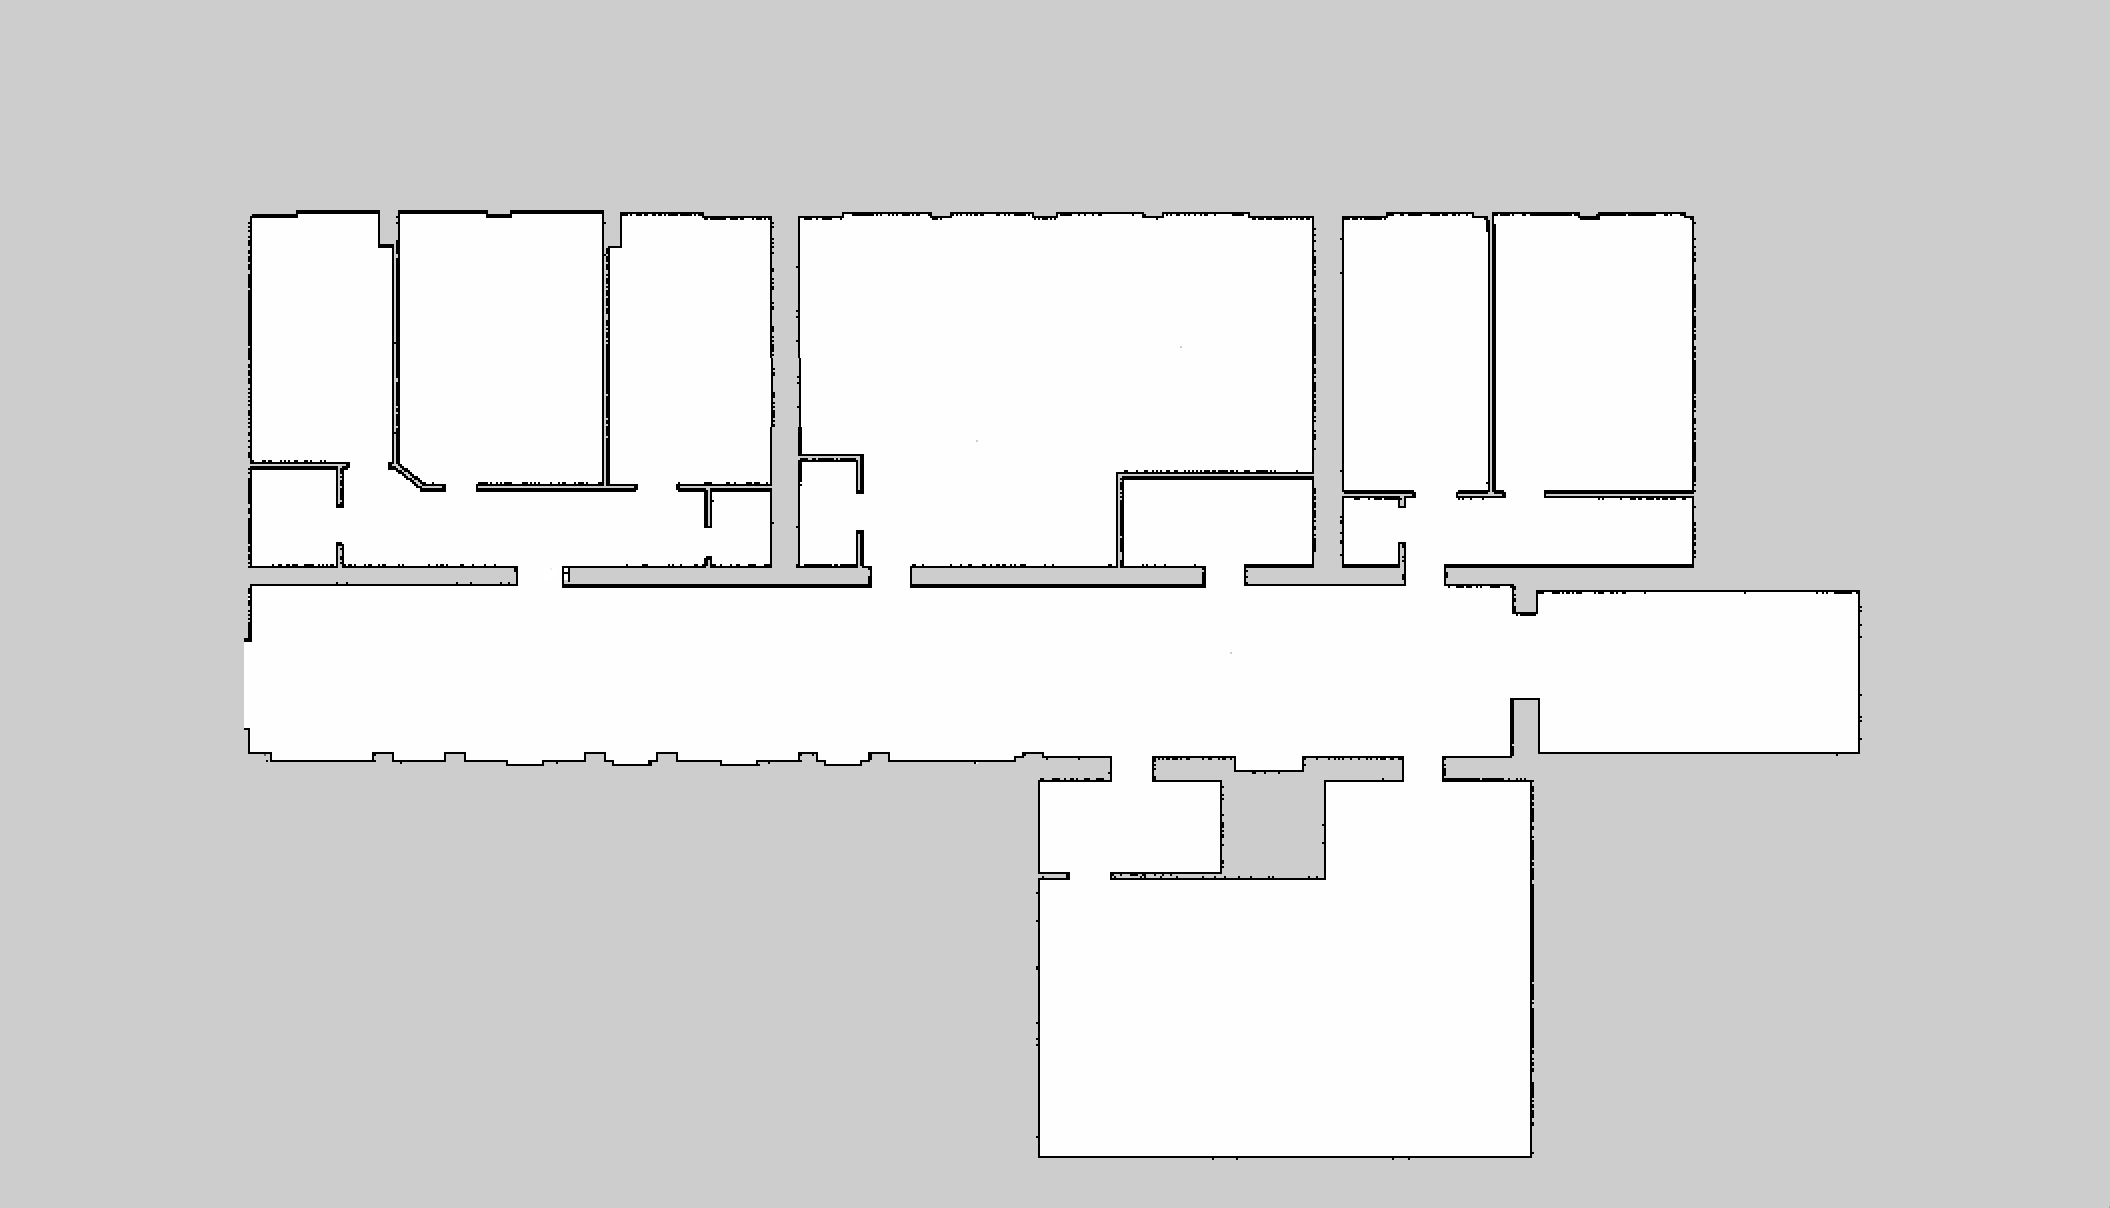
\includegraphics[width = 0.7\textwidth]{content/images/ch3/occupancy_grid.png}
	\caption{Environment occupancy grid}
	\label{fig:occupancy_grid}
\end{figure}

\section{System Environment}
A 3D Gazebo module shown in \ref{fig:gazebo_model}. It is assumed that there are no dynamic obstacles. As is shown in \ref{fig:occupancy_grid}, the black lines are occupied area, which is the wall in 3D-Model. The gray area is unknown are. 
The white area is unoccupied. In unoccupied area there are following important area and coordinates:
\begin{itemize}
	\item \textsl{Rooms.} The rectangle areas (Figure \ref{fig:room_division}) are used to represent Rooms. Each rectangle has its upper and lower limit in x and y coordinates, in order to identify which rooms the robots or targets belong to. 
	\item \textsl{Doors} The positions of doors (Figure \ref{fig:positions_door_station}) are stored in database. There are used by ROS door simulator nodes, which broadcast thier position and door status periodically. The broadcast messages are received and filtered by robots.
	\item \textsl{Charging Stations} The positions of charging stations are used by ROS charging station nodes. For details please refer to Section \ref{sec:charging_station}.
\end{itemize}

\begin{figure}[htbp]
	\centering
	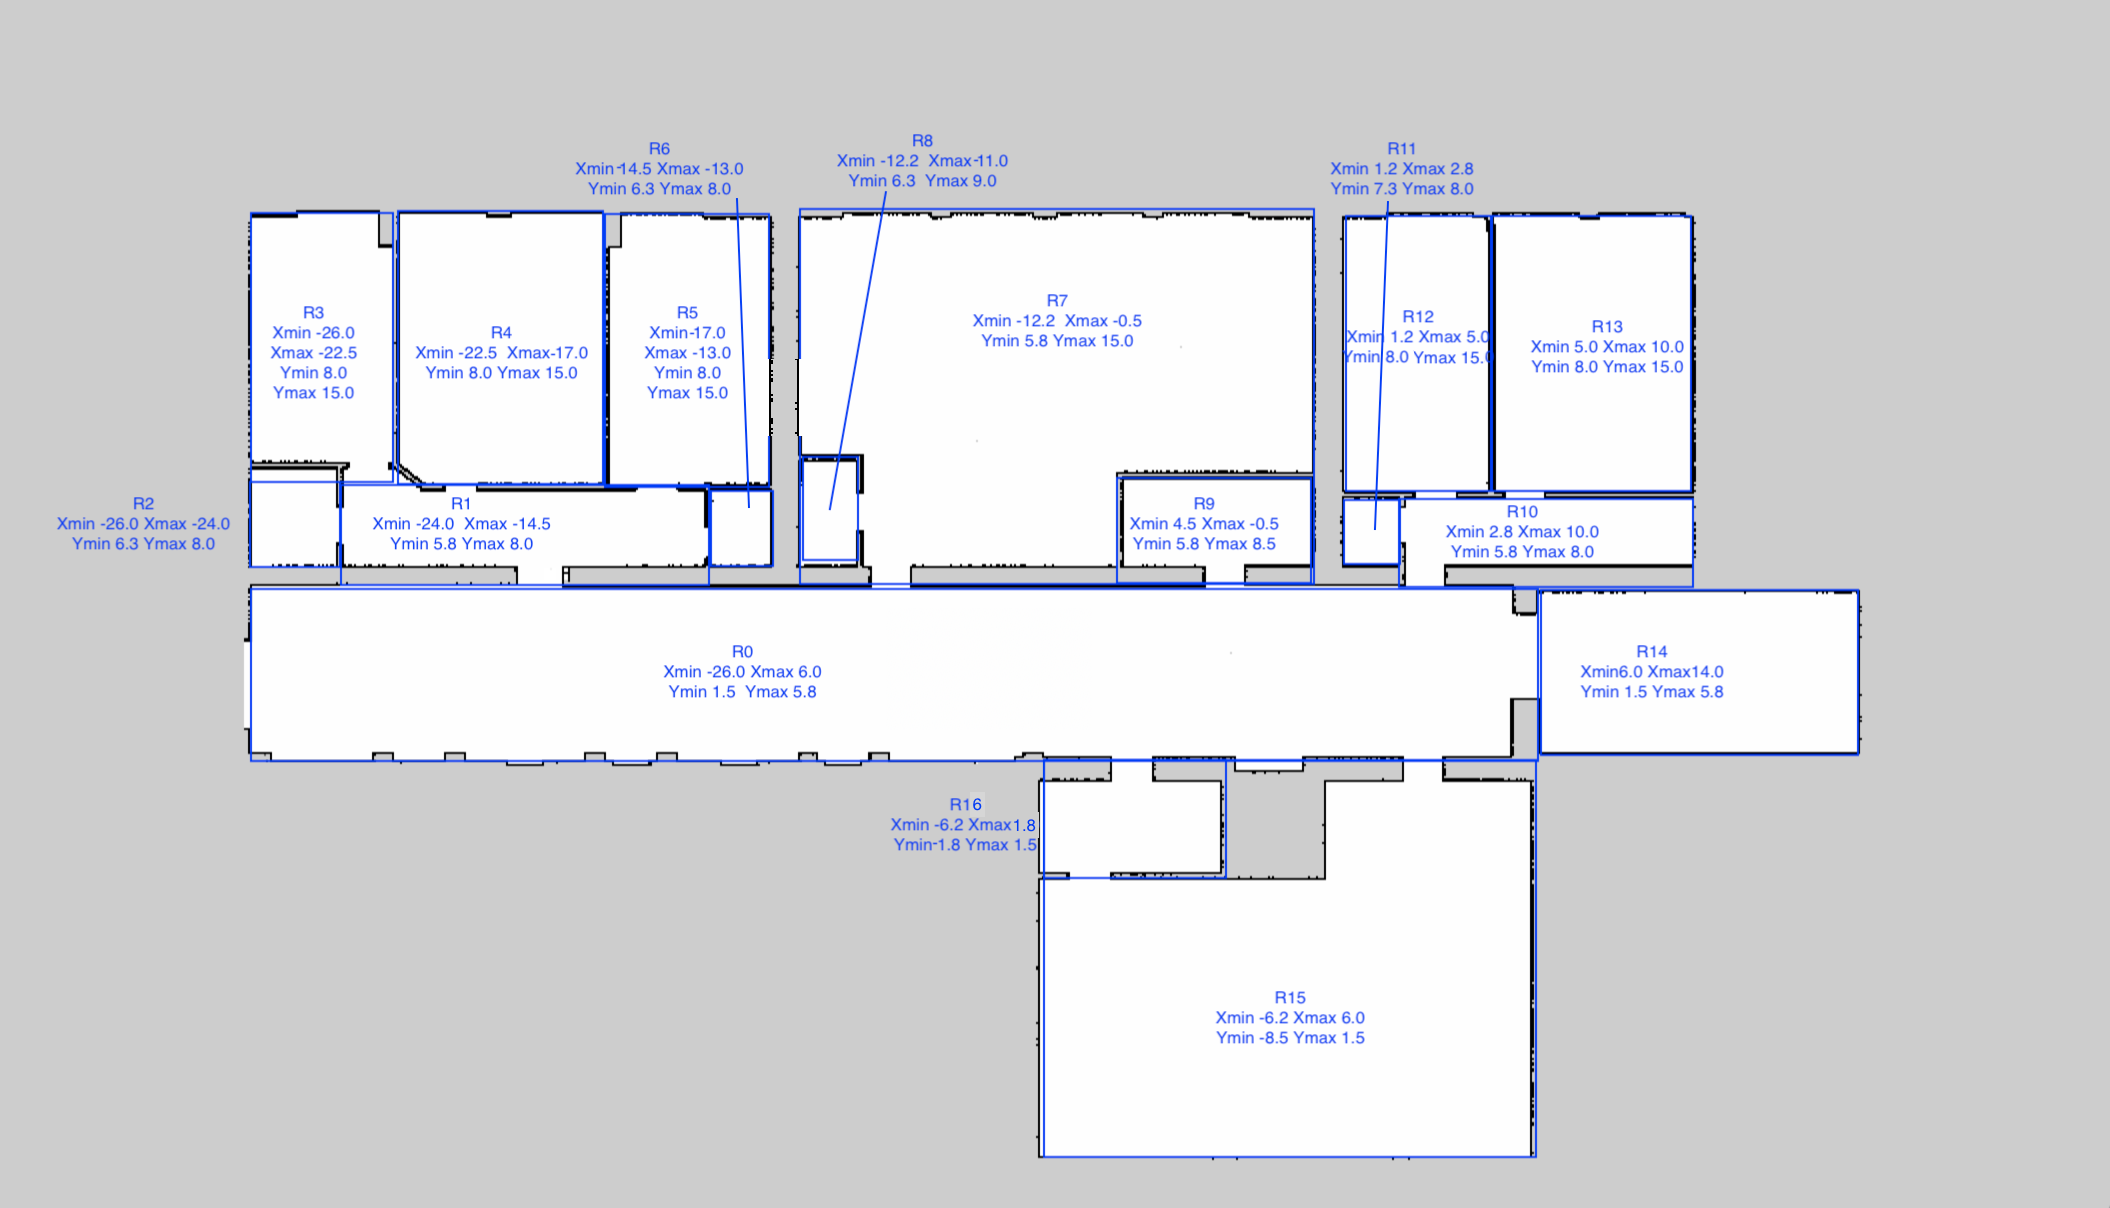
\includegraphics[width = 0.7\textwidth]{content/images/ch3/room_division.png}
	\caption{Room division}
	\label{fig:room_division}
\end{figure}

\begin{figure}[htbp]
	\centering
	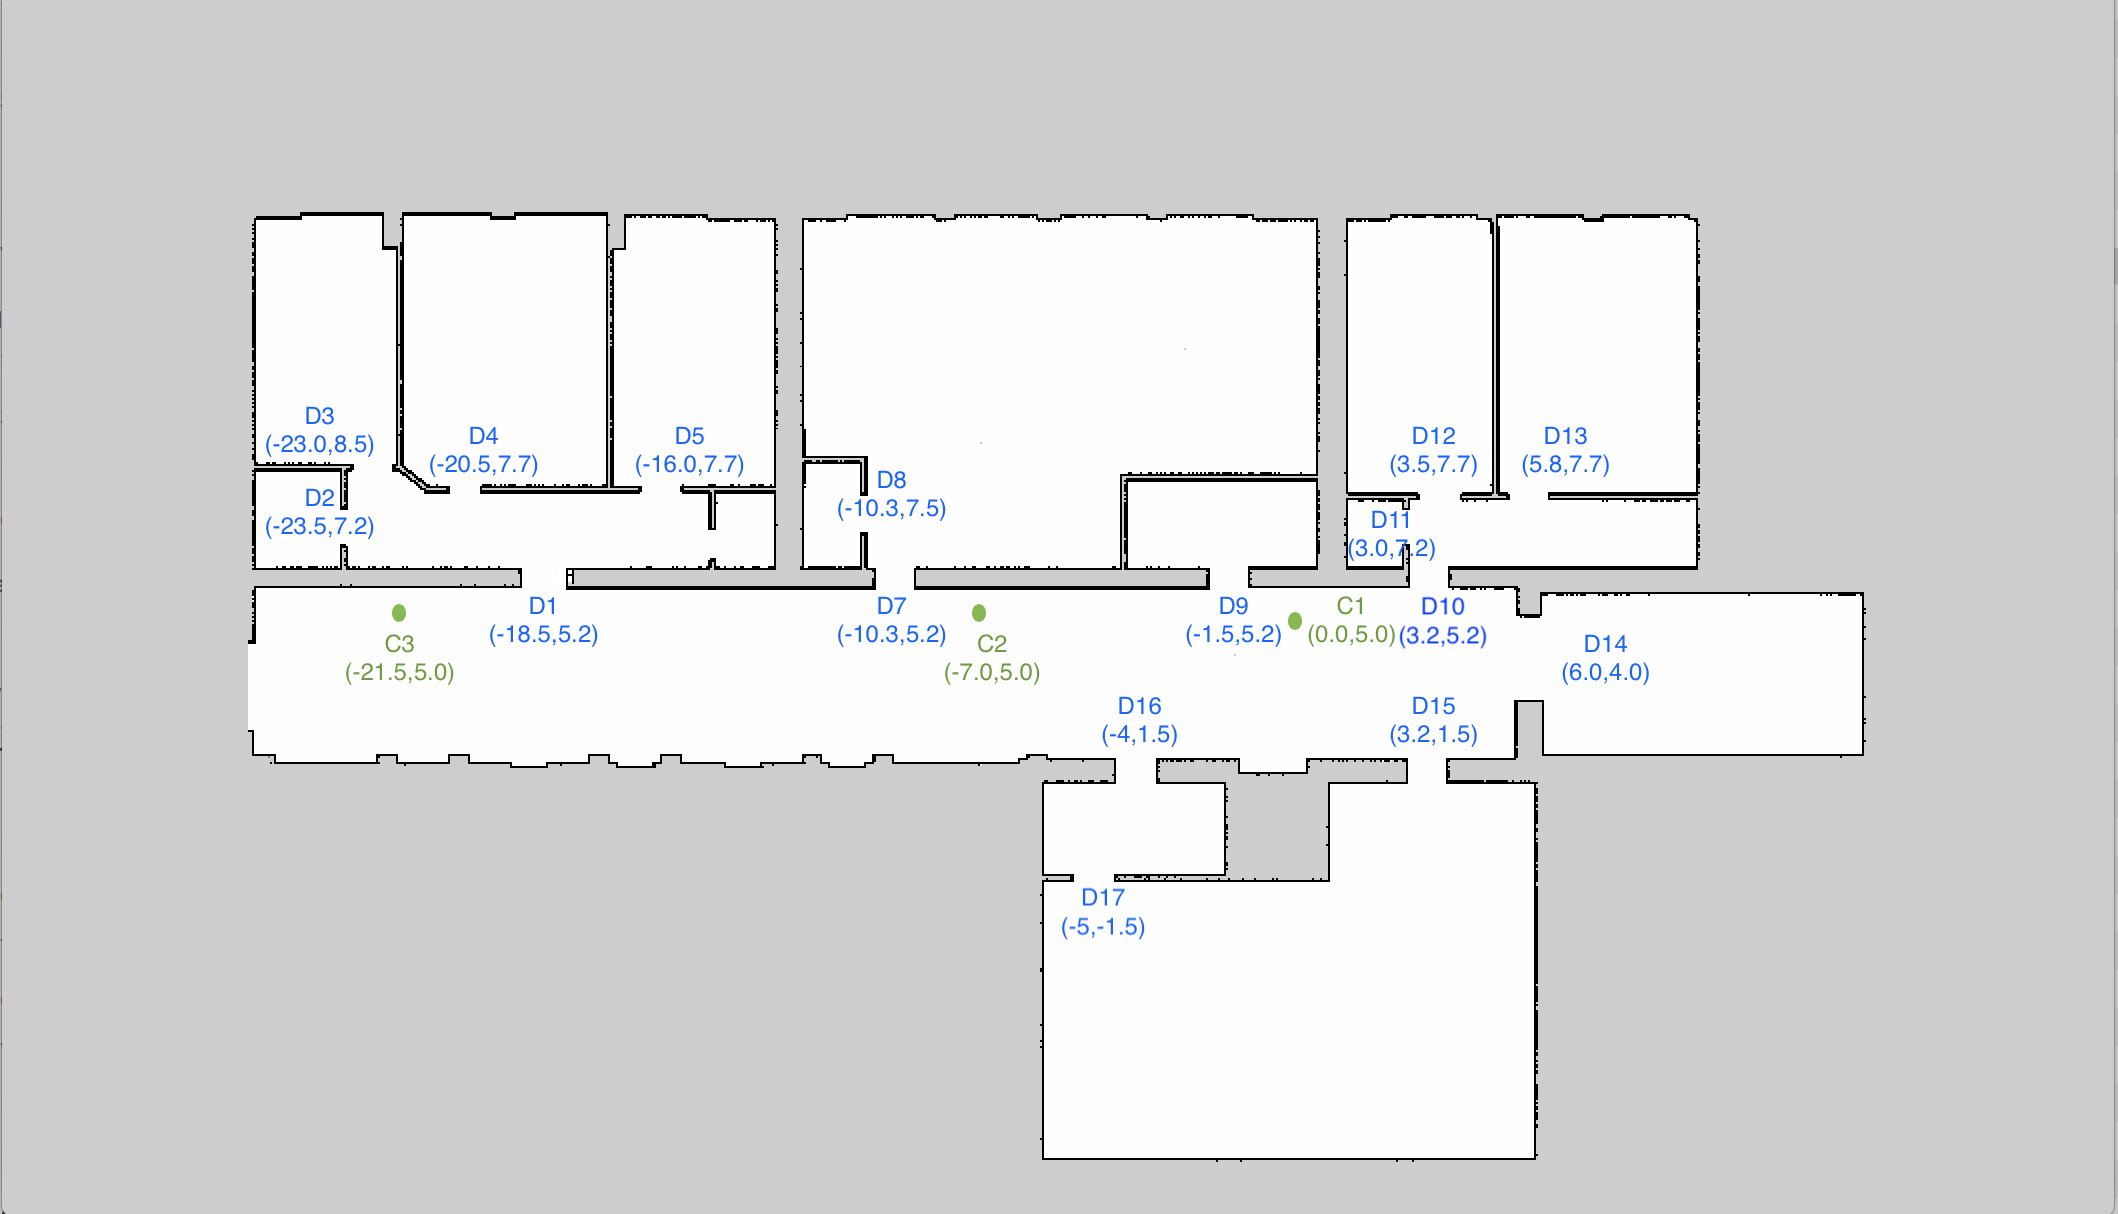
\includegraphics[width = 0.7\textwidth]{content/images/ch3/positions_door_station.png}
	\caption{Doors and Charging Stations}
	\label{fig:positions_door_station}
\end{figure}

\section{Task Allocation}

\subsection{Task Specifications}
\label{sec:task_specifications}
In order to improve overall execution efficiency, one single robot can carry either small task, which make robot move to one position, or large task, which consist of multiple small task.
On one hand, to make robot work long hours in office environment, recharging is necessary. On the other hand, a robot should gather environment information as much as possible, which centralized pool would learn from and make better decision. 
Therefore, three types of task are defined, which are shown in Table \ref{tab:task_attributes_difference} and Table \ref{tab:task_attributes_common}.  Task attributes includes task type, target, size, dependency, priority, generator, the way of handle task, start time, finish time.

\begin{table}[htb]
\centering
\resizebox{\textwidth}{!}{
\begin{tabular}{|c|c|c|c|c|c|c|c|c|c|} 
\hline
Task Attribute & Target & Dependency & Priority & Generator \\
\hline
GatherEnvironmentInfo & Door &  No & 1 & Centralized Pool\\
\hline
Execute task & Any point & Dependent on Execute-task & 2,3,4 & User\\
\hline
Charging & Charging station & No & 5 & Centralized Pool\\ [1ex] 
\hline
\end{tabular}}
\caption{Task arributes part 1}
\label{tab:task_attributes_difference}
\end{table}

\begin{table}[htb]
\centering
\resizebox{\textwidth}{!}{
\begin{tabular}{|c|c|c|} 
\hline
Task Attributes	& Start time &	Finish time \\
\hline
Explanation	& The time when robot start moving &	The time when robot finished interacting with the target \\ [1ex] 
\hline
\end{tabular}}
\caption{Task attributes part 2}
\label{tab:task_attributes_common}
\end{table}


\begin{table}[htb]
\centering
\resizebox{\textwidth}{!}{
\begin{tabular}{|c|c|c|c|c|c|c|c|c|c|} 
\hline
Task Id & Task Type & Start Time & Target Id & Robot Id & Priority & Status & dependency & Finish Time  & Description \\
\hline
1 & 2 & 10:00:00 & 10:59:59 & 0.80 & 2 & RanToCompletion & 0 & 2020-06-01 9:00:00 & Succeeded\\ [1ex] 
\hline
\end{tabular}}
\caption{Task Table in Database}
\label{tab:task_table}
\end{table}

\begin{itemize}
	\item \textsl{Task Size.} One single robot is able to carry out one Charging-task or gather environment information task, but can carry multiple Execute-task, thereby 
	These tasks with dependencies also referred to as small task. The example of small task includes Charging-task and gather environment info task. 
	Those small tasks form a dependency chain, also referred to as a large task. Execute task can be a large task which let the robot move continuously to several positions.
	\item \textsl{Target.} Targets include door, point and charging station. When a robot run a gather environment information task, it moves to the front of the door and interact with a sensor in door position, without entering the door. 
	When robot run an Execute-task, the robot moves to a given point ether in corridor or in the room.
	When robot run a Charging-task, the robot moves to charging station and interact with charging station.
\end{itemize}

\subsection{Execute Task Allocation}
\label{sec:task_allocation}
With robot information such as positions and available battery provided by robot controller, the multi-robot task allocation module in the architecture should perform multi-robot task allocation. To select an Execute-task, the following decision variable are considered.
\paragraph*{Decision variable}


\begin{table}[htb]
\centering
\begin{tabular}{|c| c| c|} 
\hline
Door Id & Door Status & Date Time \\
\hline
1& 1 & 2020-06-01 09:00:01 \\ [1ex] 
\hline
\end{tabular}
\caption{Measurement Result}
\label{tab:measurement_result}
\end{table}

\begin{table}[htb]
\centering
\resizebox{\textwidth}{!}{
\begin{tabular}{|c|c| c| c| c| c|} 
\hline
Door id & Day Of Week & Start Time & End Time & Init Open Possibility &  Open Possibility Statistic \\
\hline
1 & 2 & 10:00:00 & 10:59:59 & 0.80 & 0.80 \\ [1ex] 
\hline
\end{tabular}}
\caption{Door Open Possibility}
\label{tab:open_possibilities}
\end{table}

\begin{itemize}
\item \textsl{Task Priority.} Task priority. Task priority is an important factor that describes task emergency level. The Charging-task has the highest priority of 5. The gather environment task has the lowest priority of 1. 
	The Execute-task is determined by users but must be in the range of [2,4]. 
\item \textsl{Product of Door Open Possibility.} Because of the limitation of simulation, the door open possibility is used to represent room occupancy. The door open possibility is based on the statistic of door measurement in a specific time period of each working day. 
	The doors that the robot may pass through can be obtained from the map information module.
	An example of door measurement result is shown in Table \ref{tab:measurement_result}, an example of door open possibility table is shown in Table \ref{tab:open_possibilities}. 
\item \textsl{Waiting Time. } The waiting time is the difference of current system simulation time and start time of the first task to be executed. $T_{waiting} = T_{first\_task} - T_{now}$
\item \textsl{Battery Consumption.} The Battery Consumption is related to robot trajectory. If a robot get a Large Execute-task that contains n small task, Equation \ref{eq:battery_consumption} can be used to calculate battery consumption. The centralized pool will send the task with the lowest cost to this robot.
\end{itemize}
\begin{equation}
\begin{aligned}
\label{eq:battery_consumption}
&B: Battery\_Consumption W: Weight\\
B_{large\_task} & = \sum_{task_0}^{task_n} B_{trajectory} \\
& = \sum_{task_0}^{task_n} \sum_{waypoint_0}^{pont_M} [W_{position} \times position\_variation+W_{angle}  \times angle\_variation]\\
& = \sum_{t = task_0}^{task_n} \sum_{p = waypoint_0}^{waypoint_M} [ W_{position} \times \sqrt{(x_p-x_{p-1} )^2+(y_p-y_{p-1} )^2} \\
&   + W_{angle} \times 2 \times \arccos(w_p)] 
\end{aligned}
\end{equation}

In conclusion, equation \ref{eq:large_execute_task_cost} can be used to calculate cost of a large Execute-task.

\begin{equation}
	\label{eq:large_execute_task_cost}
	\begin{split}
	Cost_{Large\_execute\_task} = \frac{W_{battery} \times Battery\_consum}{n} + W_{waiting} \times Waiting\_time \\
	+ W_{possibility} \times \prod\limits_{i=1}^n Door\_open\_possibility  + W_{priority} \times Priority
	\end{split}
\end{equation}


\subsection{Environment Task Allocation}
Once robot request a task, The task allocation module select only tasks with cost below the threshold. Once either no task in database or all tasks cost above the threshold, 
the task allocation module should create a gather environment information task, in order to make more measurement result and further more improve the accuracy of door open possibility table.
To create a gather environment information task, which door should robot visit must be considered. The following factor help task allocation module to select the door.

\paragraph*{Decision variable}
\begin{itemize}
	\item \textsl{Door Last Update Time.} The last update time is decision variable related to gather environment information task.
	\item \textsl{Battery Consumption.} Similar to Execute-task allocation, the battery consumption is related to trajectory from robot to the door. Equation \ref{eq:battery_consumption} can be used to calculate battery consumption.
	\item \textsl{Whether door is used.} If another robot is going to this door, the value is 0, otherwise the value is 1.
\end{itemize}

\begin{equation}
	\label{eq:door_cost}
	\begin{split}
	Cost_{door} = \frac{W_{battery} \times Battery\_consum}{n} + W_{time} \times (T_{last\_update} - T_{now}) \\
	+ W_{possibility} \times \prod\limits_{i=1}^n Door\_open\_possibility + W_{is\_used} \times Is\_used  
	\end{split}
\end{equation}

\subsection{Charging Task Allocation}
Once the robot send task request to the centralized pool, and the centralized pool figure out this robot need charging, it should create a Charging-task for robot. Since there are multiple charging station in the system environment (As is shown in Figure \ref{fig:positions_door_station}), the centralized pool select a charging station for this robot using the following decision variable.

\paragraph*{Decision variable}

\begin{itemize}
	\item \textsl{Remain Time.} It describes how long the robot is charging now will take. 
	\item \textsl{Battery Consumption.} Similar to Execute-task allocation, the battery consumption is related to trajectory from robot to the door. Equation \ref{eq:battery_consumption} can be used to calculate battery consumption.
\end{itemize}
In conclusion, equation \ref{eq:charging_station_cost} can be used to calculate cost of a charging station. The centralized pool will generate a Charging-task to charging station with the lowest cost to robot which requests a task.

\begin{equation}
	\label{eq:charging_station_cost}
	\begin{split}
	Cost_{charging\_station} = \frac{W_{battery} \times Battery\_consum}{n} + W_{time} \times T_{remain}
	\end{split}
\end{equation}

 % + wt_wait \times waiting time + \prod\limits_{i=1}^n open possibility+wt_pri × priority
% wt_btr × battery consumption ÷ N + wt_wait × waiting time+ 


